\subsection{Définition du projet}
\label{subsec:def_projet}

Le projet SP-02 est une \gls{Fusex} bi-étage développée par l’association AéroIPSA pour la campagne \gls{C'Space} 2026.
Son objectif principal est la validation d’une technique de séparation inter-étage par aérofreinage, permettant de dissocier
deux étages sans recours à des systèmes pyrotechniques ni à des dispositifs mécaniques complexes. Ce concept exploite le
différentiel de traînée créé par le déploiement d’aérofreins pour initier la séparation de manière passive et contrôlée, tout en
assurant une transition stable entre les deux phases de vol.\\

En complément de cette expérience principale, le projet vise également la validation d’une architecture avionique complète,
comprenant :
\begin{itemize}
    \item un système de mesure inertielle, de pression statique et dynamique
    \item une chaîne d’acquisition, d’enregistrement et de télémesure ;
    \item un contrôle des événements critiques (séparation, allumage du second étage, récupération).\\
\end{itemize}

Ces systèmes permettront de corréler les résultats expérimentaux avec les simulations réalisées (\acrshort{CFD}, \acrshort{FEM}
et dynamique de vol) afin d’évaluer l’efficacité du dispositif d’aérofreinage et la stabilité de la fusée durant les différentes
phases.\\

Cette stabilité est assurée par un jeu de 8 surfaces passives (4 ailerons par étage) positionnées en queue de chaque étage.
Elles sont dimensionnées pour garantir une stabilité statique suffisante tout au long du vol de l'ensemble de la fusée ainsi que
les étages pris individuellement après séparation.\\

La stratégie de récupération de chaque étage repose sur l’ouverture de trappes latérales permettant le déploiement de
parachutes. Elles sont commandées par les séquenceurs embarqués, qui déclenchent l’ouverture à la détection de l’apogée de chaque
étage via des capteurs barométriques. Les séquenceurs des deux étages sont du même modèle, mais configurés différemment selon
les besoins spécifiques de chaque étage.\\

Le système de mesure embarqué est également conçu en double exemplaire, un pour chaque étage. Nommé \gls{APEX}, ce système a déjà
été développé et a volé avec succès 3 fois lors de la campagne de lancements du \gls{C'Space} 2025.

\newpage

\subsubsection{Premier étage}

Le premier étage de la fusée SP-02 est conçu pour fournir la poussée initiale nécessaire au lancement et à l’ascension jusqu’à la
séparation. Il intègre le système d’aérofreinage destiné à ralentir l’étage inférieur au moment de la séparation et le système de
séparation des deux étages.\\

Voici les principales caractéristiques techniques du premier étage :
\begin{itemize}
    \item Hauteur : 1120 mm
    \item Diamètre interne : 100 mm
    \item Epaisseur de paroi : 2 mm
    \item Masse à vide : 4431 g
    \item Propulseur : Cesaroni K570 - Pro54-5G Barasinga
\end{itemize}
% \vspace{-2cm}
\begin{figure}[h]
    \centering
    \begin{tikzpicture}
    
        \node at (0, 0) {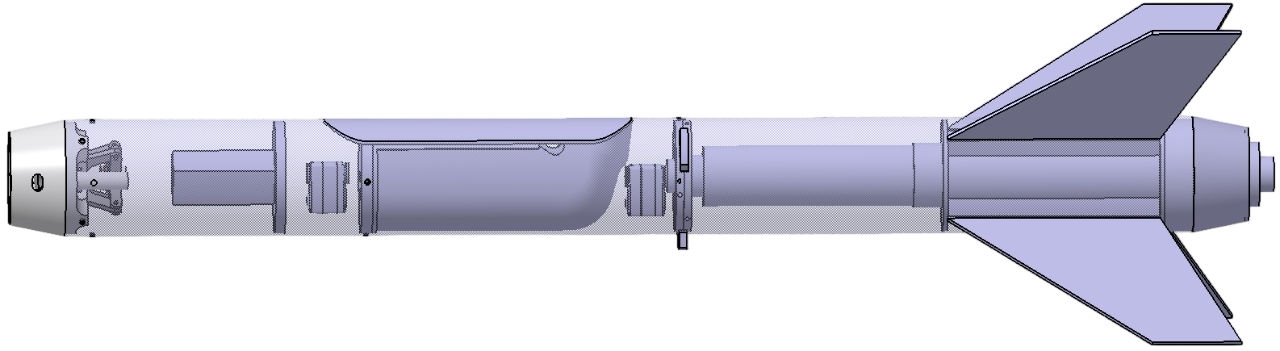
\includegraphics[width=\textwidth]{figures/catia_alpha.png}};
        
        \node (retreint_lbl)   at (+8.00, +2.5) {\textbf{Rétreint}};
        \node (bloc_propu_lbl) at (+4.30, +2.3) {\textbf{Bloc propulsion}};
        \node (propu_lbl)      at (+2.00, +1.5) {\textbf{Pro54-5G}};
        \node (aileron_lbl)    at (+2.00, -1.5) {\textbf{Ailerons (x4)}};
        \node (af_lbl)         at (+0.00, +2.3) {\textbf{Aérofreins (x3)}};
        \node (bloc_para_lbl)  at (-2.00, +1.5) {\textbf{Bloc parachute}};
        \node (bloc_elec_lbl)  at (-6.00, +2.3) {\textbf{Bloc électronique}};
        \node (bloc_sepa_lbl)  at (-6.00, -1.5) {\textbf{Bloc séparation}};

        \node (bloc_propu_box) at (+5.10, 0.00) [minimum width=35mm, minimum height=18mm, rectangle, line width=2, draw=red] {};
        
        \draw[red, ->, line width=1.5] (retreint_lbl.south)   -- (+7.20, +0.60);
        \draw[red, ->, line width=1.5] (bloc_propu_lbl.south) -- (bloc_propu_box.140);
        \draw[red, ->, line width=1.5] (propu_lbl.south)      -- (+2.20, +0.00);
        \draw[red, ->, line width=1.5] (aileron_lbl.east)     -- (+6.50, -1.50);
        \draw[red, ->, line width=1.5] (af_lbl.south)         -- (+0.30, +0.60);
        \draw[red, ->, line width=1.5] (bloc_para_lbl.south)  -- (-2.00, +0.00);
        \draw[red, ->, line width=1.5] (bloc_elec_lbl.south)  -- (-5.30, +0.00);
        \draw[red, ->, line width=1.5] (bloc_sepa_lbl.north)  -- (-7.30, +0.00);

    \end{tikzpicture}
    \caption{Vue du premier étage sur \acrshort{CATIA}}
    \label{fig:sp02_s1_ork}
\end{figure}

\subsubsection{Deuxième étage}

Le deuxième étage de la fusée SP-02 est conçu pour assurer la sécurité de l'allumage du moteur après la séparation et pour
fournir la poussée nécessaire à l'atteinte d'une altitude supérieure à celle du premier étage. Il est également équipé d'un tube
pitot.\\

Voici les principales caractéristiques techniques du deuxième étage :
\begin{itemize}
    \item Hauteur : 992 mm
    \item Diamètre interne : 80 mm
    \item Epaisseur de paroi : 2 mm
    \item Masse à vide : 2895 g
    \item Propulseur : Cesaroni G150 - Pro24-6G Pandora
\end{itemize}
\begin{figure}[h]
    \centering
    \begin{tikzpicture}
    
        \node at (0, 0) {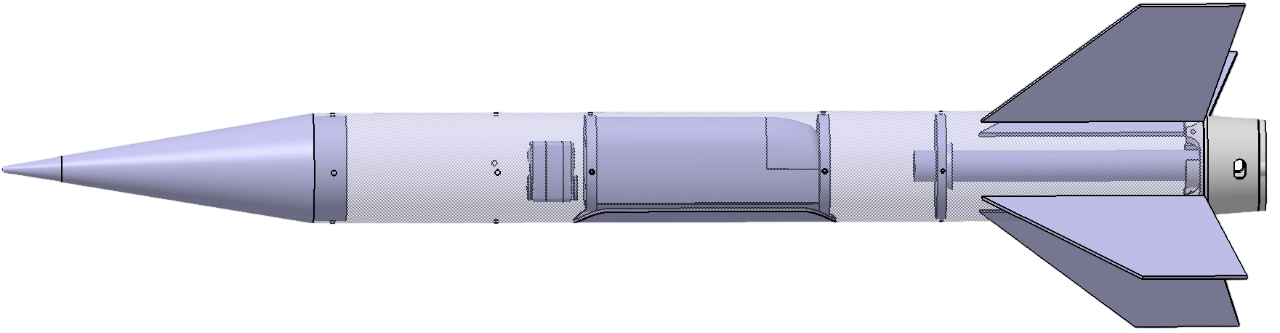
\includegraphics[width=\textwidth]{figures/catia_beta.png}};
        
        \node (bloc_sepa_lbl)   at (+8.00, +2.5) {\textbf{Interface de séparation}};
        \node (propu_lbl)       at (+4.30, +2.3) {\textbf{Pro24-6G}};
        \node (bague_propu_lbl) at (+3.00, +1.5) {\textbf{bague de centrage}};
        \node (aileron_lbl)     at (+2.00, -1.5) {\textbf{Ailerons (x4)}};
        \node (bloc_para_lbl)   at (+1.00, +2.3) {\textbf{Bloc parachute}};
        \node (bloc_elec_lbl)   at (-2.00, +1.5) {\textbf{Bloc électronique}};
        \node (coiffe_lbl)      at (-5.00, +2.3) {\textbf{Coiffe conique}};
        \node (pointe_alu_lbl)  at (-6.00, -1.5) {\textbf{Pointe aluminium}};

        \draw[red, ->, line width=1.5] (bloc_sepa_lbl.south)    -- (+7.40, +0.60);
        \draw[red, ->, line width=1.5] (propu_lbl.south)        -- (+5.20, +0.00);
        \draw[red, ->, line width=1.5] (bague_propu_lbl.south)  -- (+3.70, +0.00);
        \draw[red, ->, line width=1.5] (aileron_lbl.east)       -- (+6.50, -1.00);
        \draw[red, ->, line width=1.5] (bloc_para_lbl.south)    -- (+0.30, +0.60);
        \draw[red, ->, line width=1.5] (bloc_elec_lbl.south)    -- (-2.50, +0.00);
        \draw[red, ->, line width=1.5] (coiffe_lbl.south)       -- (-5.30, +0.00);
        \draw[red, ->, line width=1.5] (pointe_alu_lbl.north)   -- (-7.30, +0.00);

    \end{tikzpicture}
    \caption{Vue du second étage sur \acrshort{CATIA}}
    \label{fig:sp02_s2_ork}
\end{figure}

\newpage

\subsubsection{Ensemble de la fusée}

L’ensemble de la fusée SP-02, une fois les deux étages assemblés, présente les caractéristiques suivantes :
\begin{itemize}
    \item Hauteur totale : 2052 mm
    \item Diamètre externe : 104 mm
    \item Masse à vide : 7327 g
\end{itemize}

\begin{figure}[h]
    \centering
    \rotatebox{-75}{
        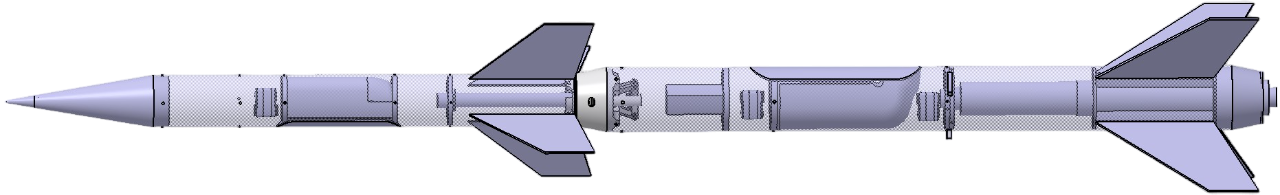
\includegraphics[width=0.9\textwidth]{figures/catia_alpha_beta.png}
    }
    \caption{Vue d'ensemble de la fusée SP-02 sur \acrshort{CATIA}}
    \label{fig:sp02_ork}
\end{figure}


\subsubsection{Choix des propulseurs}

Le choix des propulseurs pour les deux étages de la fusée SP-02 a été effectué en tenant compte de deux critères clés qui sont
les objectifs de la mission et l'accessibilité des moteurs. Le premier étage utilise un moteur Cesaroni K570 - Pro54-5G Barasinga,
tandis que le deuxième étage est propulsé par un moteur Cesaroni G150 - Pro24-6G Pandora. Ces moteurs ont été les plus accessible
lors des \gls{C'Space} précédentes et offrent des performances suffisante à l'atteinte des objectifs de la mission. En effet,
aucune exigence importante d'atteindre une altitude spécifique n'a été définie. Seule la vitesse lors de la séparation des deux
étages doit être suffisante pour garantir le bon fonctionnement du système d'aérofreinage.\\

\newpage